\section{Neuronal views and display selection}
\label{sec:s:views}

\paragraph{Illustrative unequal-peak example.}
The main neuronal figure uses SOM006\_cell3\_c0 with pretrained PnP at $C=8$ and nominal dose. We screened the 60 references for interior columns with exactly two peaks, separated by at least three planes, and a weaker-to-stronger height ratio of 0.2--0.6. Peaks must meet the height and prominence thresholds used for layered-column evaluation. A supported region contains the center and at least four neighboring eligible columns with corresponding peak planes within one plane. This gives 685 eligible columns and 13 supported regions in six crops. An expanded screen with two supporting neighbors was also examined; the selected column meets the original, stricter rule. We inspected paired reconstruction outcomes and selected the displayed column for its lower W1 and better retention of the weaker component across all five subsets. This is an outcome-selected local illustration, not a representative or aggregate comparison.

The column is $(x,y)=(35,30)$, with reference peaks at planes 3 and 11 (zero-based) and a weaker-to-stronger height ratio of 0.59. The axial band spans rows 34--36. \Cref{tab:s:unequalpeaks,fig:s:unequalpeaks} give the five-subset errors and profiles, including raw intensity. Our column W1 is lower than both controls in every subset. Among the 13 original region centers, our and end-to-end W1 beat the untrained plate in all five subsets at 10 and 8 centers, respectively; each learned plate beats both others at one center. The larger region around the displayed column does not share its ordering: our and end-to-end mean W1 are $0.223$ and $0.210\um$ over its five columns, and $0.220$ and $0.218\um$ over the crop. The displayed volumes reproduce the recorded rows within $0.002$\,dB PSNR and $0.0003\um$ crop W1.

\begin{table}[t]
\centering\small
\begin{tabular}{lrrr}
\toprule
Subset & Untrained & Ours & End-to-end \\
\midrule
1 & 0.344 & 0.117 & 0.231 \\
2 & 0.514 & 0.110 & 0.366 \\
3 & 0.490 & 0.102 & 0.147 \\
4 & 0.648 & 0.150 & 0.296 \\
5 & 0.815 & 0.169 & 0.346 \\
\midrule
Mean & 0.562 & \textbf{0.130} & 0.277 \\
\bottomrule
\end{tabular}
\caption{Column W1 ($\mu$m) for the selected unequal-peak example across the five recorded direction subsets. Subset 1 is displayed in the main figure.}
\label{tab:s:unequalpeaks}
\end{table}

\begin{figure*}[t]
\centering
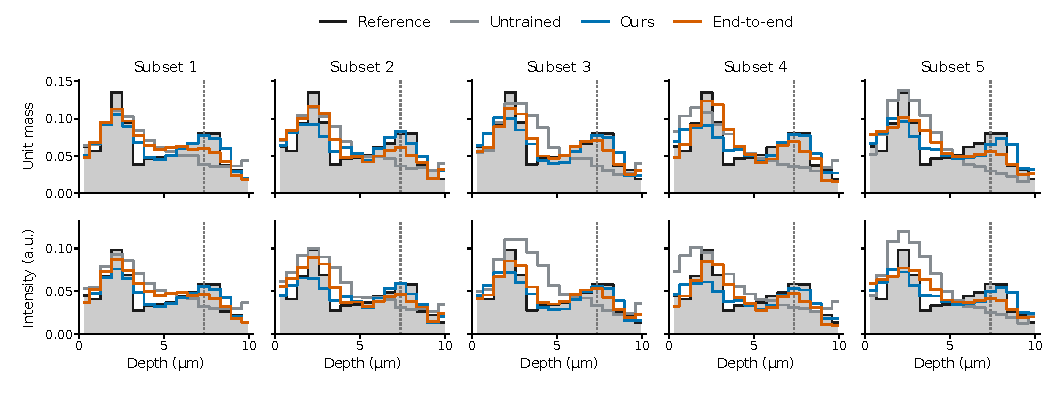
\includegraphics[width=\linewidth]{unequal_peak_profiles.pdf}
\caption{The selected main-figure column across all five direction subsets. Top: unit-mass axial profiles used for column W1. Bottom: raw intensities on one shared linear scale. Gray fills show the reference, and the dashed line marks its weaker peak. Our plate preserves this component's relative strength more closely across subsets; in Subset 1, it also underestimates the stronger peak most.}
\label{fig:s:unequalpeaks}
\end{figure*}

\paragraph{Reference-only selection.}
Before opening reconstructions for figure selection, we computed reference features for all 60 crops. Eligible crops had at least 10 skeleton endpoints (the upper quartile) and a 10--90\,\% column-centroid range of at least $3.64\um$ (the median), indicating several branches and substantial depth extent. Eight crops qualified. We ranked them by reference signal in columns with at least two axial peaks. The first was SOM004\_cell2\_x7; the companion was the highest-ranked eligible crop from another animal, SOM006\_cell1\_x7.

After selection, their W1-gain ranks among 60 crops were 52/45/23 and 45/46/43 for TV/pretrained/neuron-trained PnP, where rank 1 is the largest reduction. These are typical-to-lower-gain examples. We retain both alongside the main figure's unequal-peak illustration. \Cref{fig:s:mainviews,fig:s:companion} show all three iterative methods for these crops. The full-cell panels supply two-photon context; only the marked crops generate simulated measurements.

\paragraph{Views and scales.}
For the two reference-selected crops, the axial band maximizes reference signal in layered columns over three consecutive lateral rows ($1.92\um$). Within it, the profile column has the largest reference signal among layered columns whose two highest peaks are at least three planes apart. This gives $(x,y)=(35,44)$ in the first crop and $(42,16)$ in the companion; the first lies three voxels from an edge and was retained unchanged. Their displayed volumes use noise draw 0. These columns favor the end-to-end plate more strongly than the crop-wide error; they illustrate local behavior, not a population ranking.

Depth-colored projections tint each plane with an approximately constant-lightness depth color at its linear intensity, then take the maximum independently in each color channel. Overlapping layers may mix colors or be dominated by the brighter layer, so axial bands, profiles and W1 maps accompany the projections. Fluorescence intensity images---bands, slabs, reference projections and two-photon contexts---use inverted gray, so darker pixels carry more signal. Reconstruction panels use one linear range per crop, from zero to the 99.5th percentile of its reference maximum projection, with no gamma, smoothing or per-panel rescaling. W1 maps use a shared 0--$1\um$ scale from light pink at zero to deep purple at or above $1\um$; white marks unscored pixels outside the reference signal mask. Rows and columns correspond to $x$ and $y$ throughout; axial depth increases downward.

Full-cell contexts are maximum projections of the original two-photon stacks, linearly clipped at their 99.8th percentile. They retain tissue coordinates ($0.25\um$ lateral sampling), whereas reconstructed views use simulation coordinates. The boxed $32\times32\times32\um^3$ tissue crops become $30.72\times30.72\times10.24\um^3$ simulated volumes. The reference-selected reconstructions reproduce the recorded rows within $0.018$\,dB PSNR and $0.001\um$ W1. The following full views retain context and individual profiles.

\begin{figure*}[t]
\centering
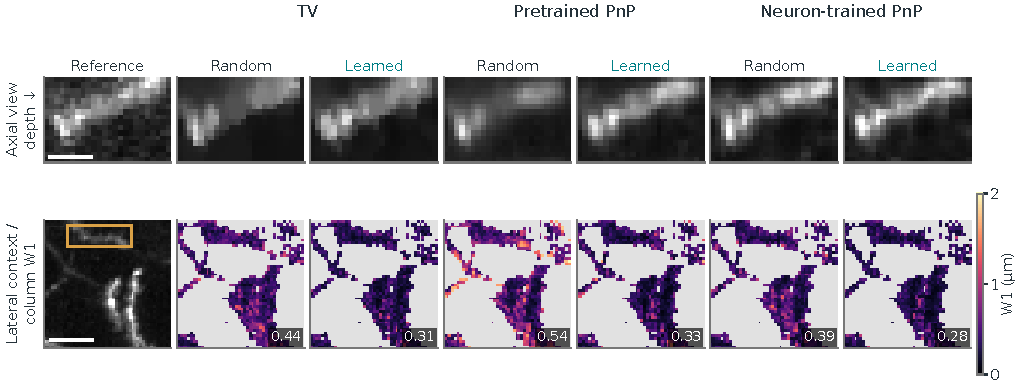
\includegraphics[width=\linewidth]{neuron_comparison.pdf}
\caption{All three iterative methods for the first reference-selected crop. Left: matched axial bands for the reference, untrained, our and end-to-end plates. Right: column-W1 maps with draw-0 crop means below. White marks pixels outside the reference signal mask. The $5\um$ bar applies to both axes of each band; maps span the full $30.72\um$ lateral field.}
\label{fig:s:mainviews}
\end{figure*}

\begin{figure*}[t]
\centering
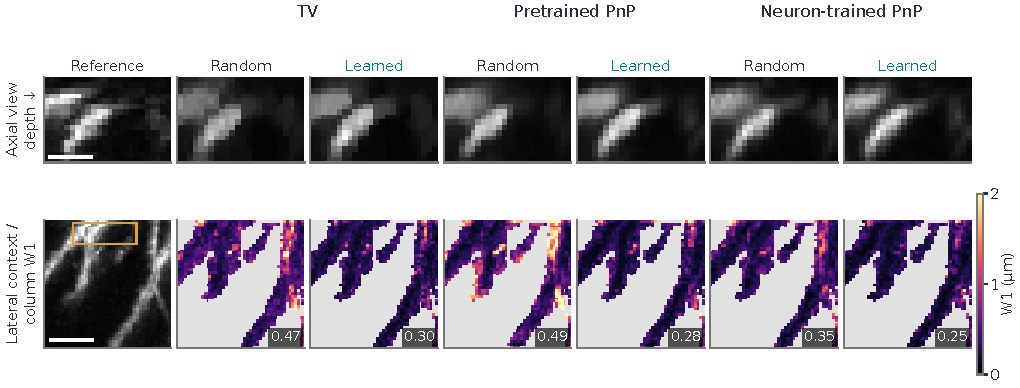
\includegraphics[width=\linewidth]{neuron_companion.pdf}
\caption{The companion crop from another animal, using the same band and error-map conventions as \cref{fig:s:mainviews}. Values are draw-0 crop W1 in $\mu$m; the bar is $5\um$.}
\label{fig:s:companion}
\end{figure*}

\begin{figure*}[t]
\centering
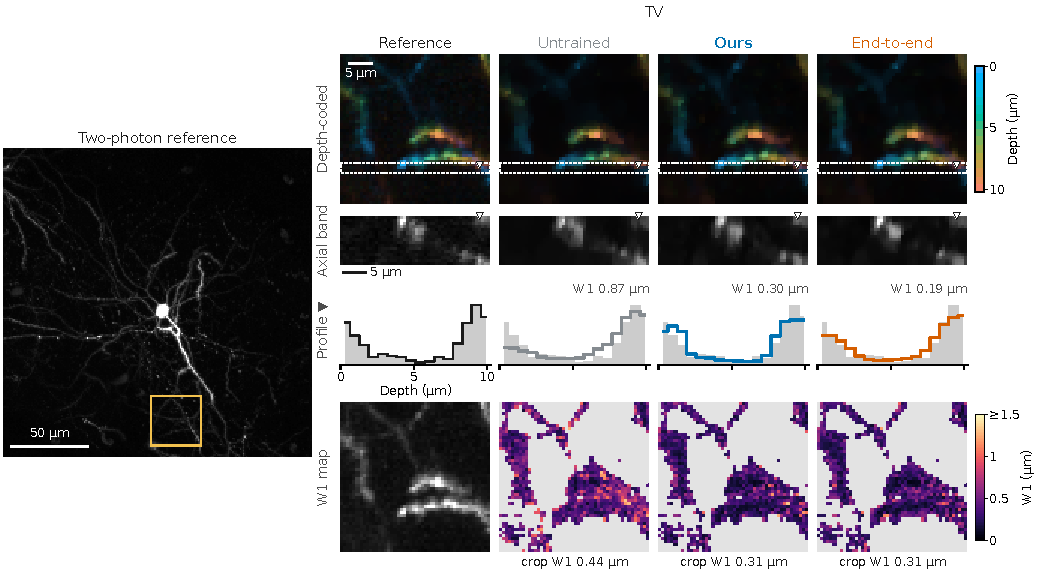
\includegraphics[width=\linewidth]{neuron_tv.pdf}
\caption{First crop with TV. Context, projection, band, profile and error-map conventions match the main neuronal figure. The marked profile is one reference-selected column; the means below the maps summarize all reference-signal columns for this draw.}
\label{fig:s:tvview}
\end{figure*}

\begin{figure*}[t]
\centering
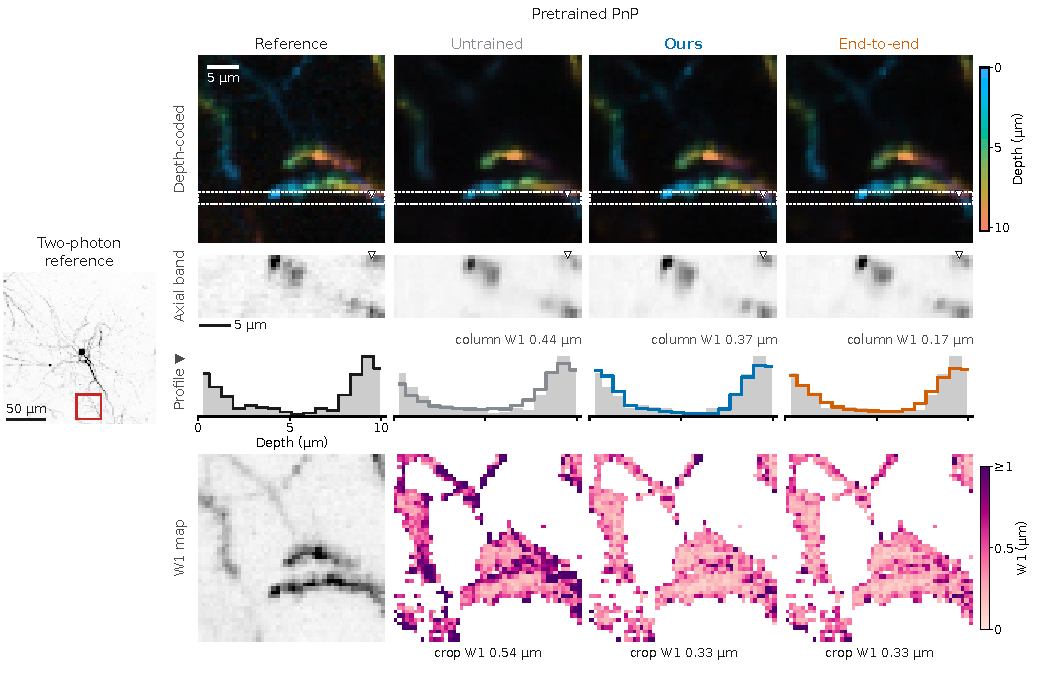
\includegraphics[width=\linewidth]{neuron_pretrained.pdf}
\caption{First reference-selected crop with pretrained PnP, retained from the earlier main figure. The marked column favors end-to-end more strongly than the crop mean.}
\label{fig:s:pretrainedview}
\end{figure*}

\begin{figure*}[t]
\centering
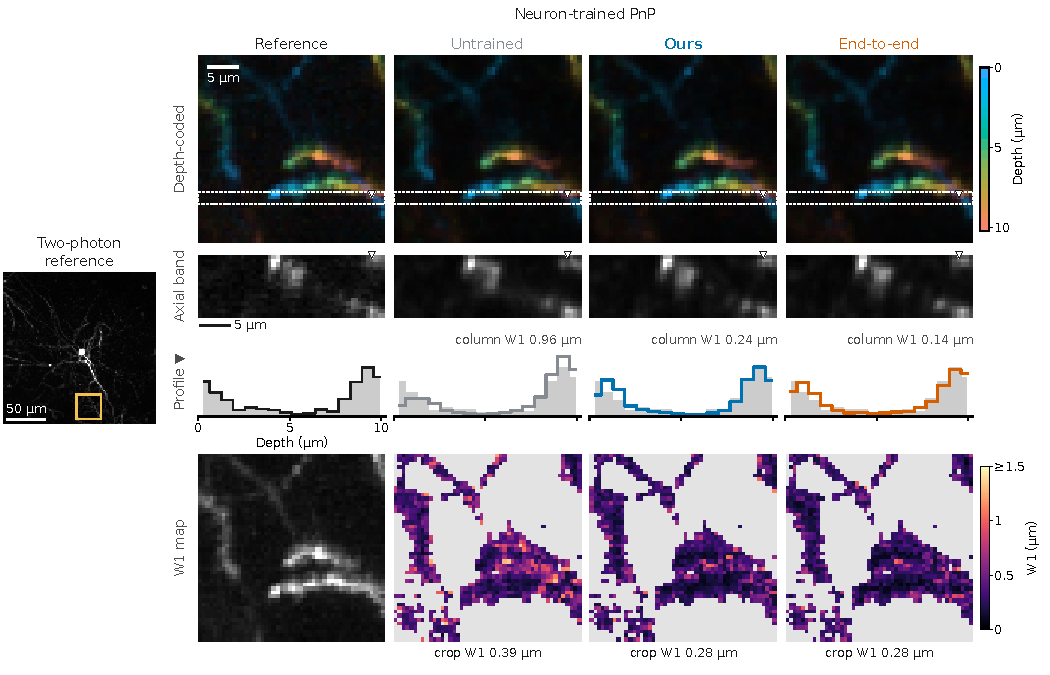
\includegraphics[width=\linewidth]{neuron_trained.pdf}
\caption{First crop with neuron-trained PnP. Context, projection, band, profile and error-map conventions match the main neuronal figure. The marked profile is one reference-selected column; the means below the maps summarize all reference-signal columns for this draw.}
\label{fig:s:neuronview}
\end{figure*}

\begin{figure*}[t]
\centering
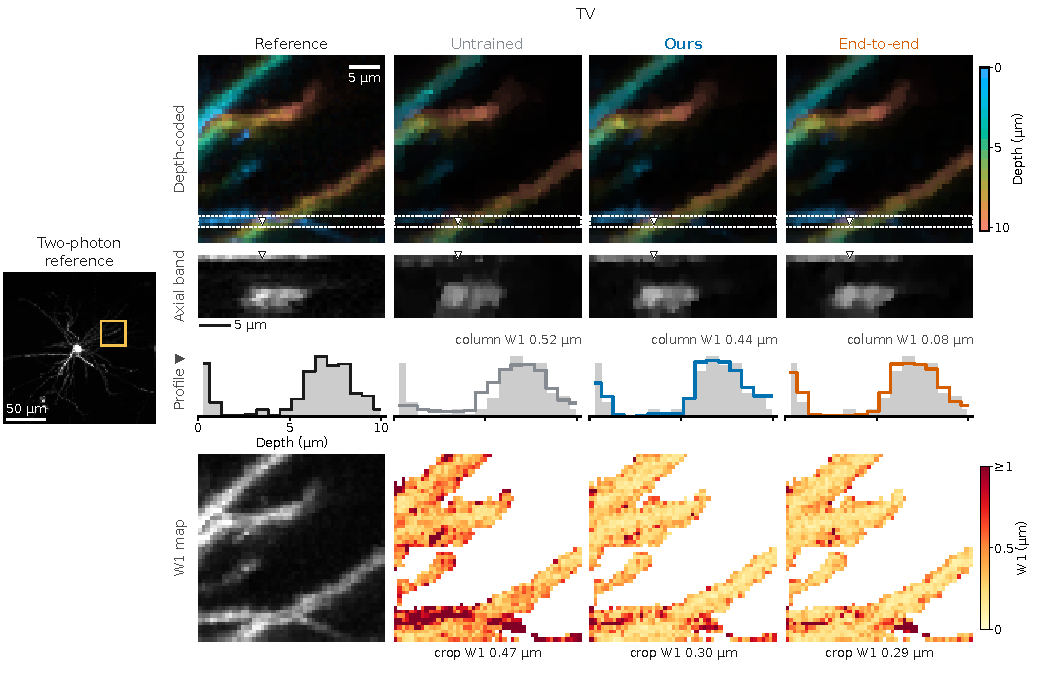
\includegraphics[width=\linewidth]{companion_tv.pdf}
\caption{Companion crop with TV. Context, projection, band, profile and error-map conventions match the main neuronal figure. The marked profile is one reference-selected column; the means below the maps summarize all reference-signal columns for this draw.}
\label{fig:s:companTV}
\end{figure*}

\begin{figure*}[t]
\centering
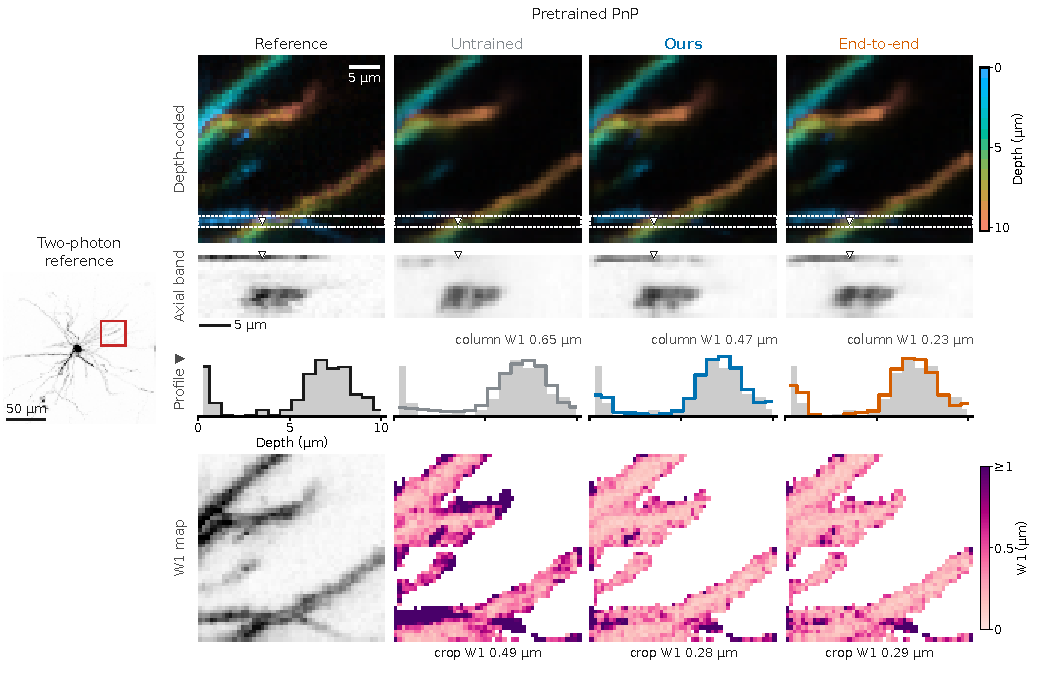
\includegraphics[width=\linewidth]{companion_pretrained.pdf}
\caption{Companion crop with pretrained PnP. Context, projection, band, profile and error-map conventions match the main neuronal figure. The marked profile is one reference-selected column; the means below the maps summarize all reference-signal columns for this draw.}
\label{fig:s:companPre}
\end{figure*}

\begin{figure*}[t]
\centering
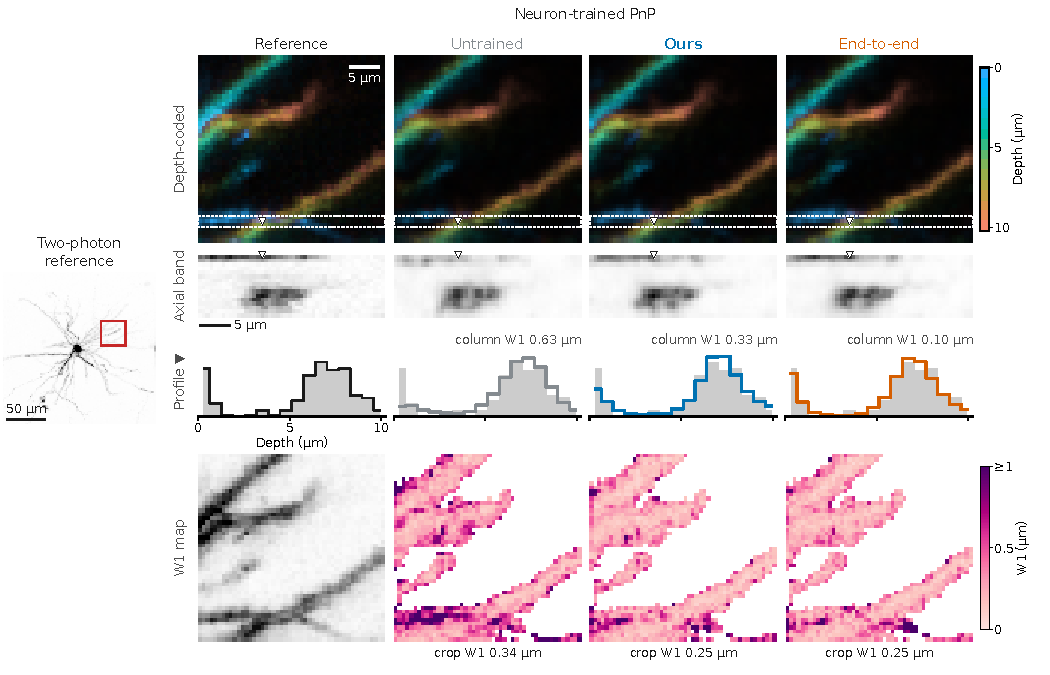
\includegraphics[width=\linewidth]{companion_trained.pdf}
\caption{Companion crop with neuron-trained PnP. Context, projection, band, profile and error-map conventions match the main neuronal figure. The marked profile is one reference-selected column; the means below the maps summarize all reference-signal columns for this draw.}
\label{fig:s:companNeur}
\end{figure*}

\begin{figure*}[t]
\centering
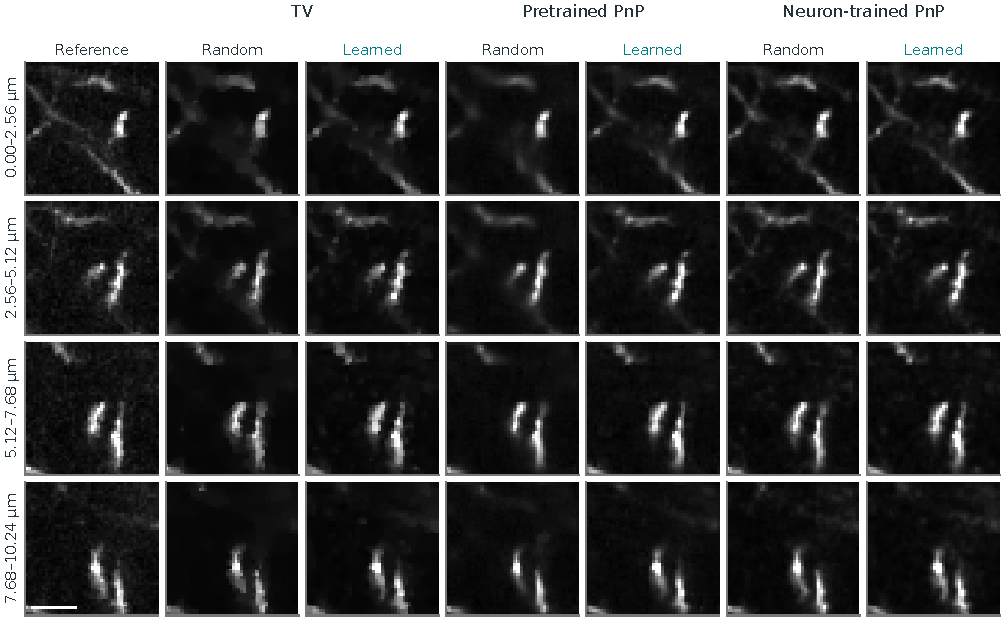
\includegraphics[width=\linewidth]{neuron_slabs_a.pdf}
\caption{Depth slabs of the first neuronal example, with maximum projections over four consecutive depth planes ($2.56\um$ per slab). Reference and all reconstructions share the same linear intensity range across slabs. Slab views expose signal spread into depths absent from the corresponding reference slab. These are qualitative placement comparisons, not branch-separation measurements. Bar: $10\um$.}
\label{fig:s:slabsa}
\end{figure*}

\begin{figure*}[t]
\centering
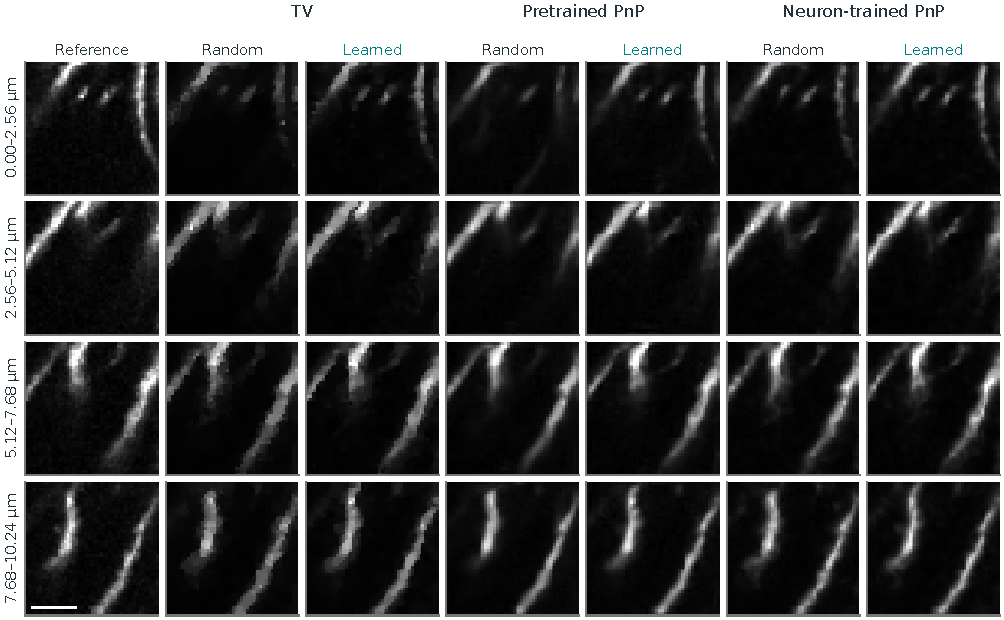
\includegraphics[width=\linewidth]{neuron_slabs_b.pdf}
\caption{The companion crop from another animal, with the same depth-slab conventions. Stronger priors reduce diffuse signal for both plates; the optical difference is smaller under neuron-trained PnP. The full views retain features missed by either encoder.}
\label{fig:s:slabsb}
\end{figure*}

\paragraph{A feature missed by both plates.}
A separate weak-feature illustration uses the earlier reference-selected companion band: the layered column with largest reference mass whose two highest peaks are at least three planes apart. Its selected column, $(x,y)=(18,3)$, contains a weak shallow peak at plane 2 above a deeper peak at plane 9. The shallow peak is 24.5\,\% of the column maximum and carries 7.8\,\% of its signal in planes 1--3. None of the six untrained- and our-plate reconstructions has a matched shallow peak; that signal becomes a low plateau (\cref{fig:s:weakprofile}). This limit coexists with lower average W1 and improved placement of brighter features.

\begin{figure*}[t]
\centering
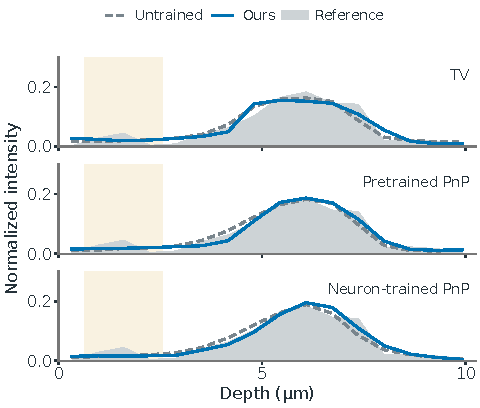
\includegraphics[width=.48\linewidth]{neuron_weak_profile.pdf}
\caption{Reference-selected weak-feature column in the companion crop. Profiles are normalized to unit mass. Both plates miss the shallow reference peak under all three priors, despite the lower average W1 of our plate. This column was fixed from reference structure before inspecting reconstructions.}
\label{fig:s:weakprofile}
\end{figure*}
